\documentclass[../main]{subfiles}
\begin{document}
\chapter{Variational Autoencoder (VAE)}
\begin{introduction}
    \item Deep generative models
    \item Autoencoder (AE)
    \item Latent-variable generative modeling
    \item Variational inference and ELBO
    \item VAE objective
    \item Reparameterization trick
\end{introduction}

% Make figures work both when compiling main.tex and when compiling this chapter alone.
\graphicspath{{tikz/}{../tikz/}{../../tikz/}{../../mvp/tikz/}}

In the previous chapter, we have already seen latent-variable models such as
Mixture of Gaussians (MoG), whose generative story is explicit and simple.  
However, realistic data distributions (e.g.\ natural images) are far more complex:
\begin{itemize}
    \item Images live in an extremely high-dimensional space (e.g.\ a $256\times256$ RGB image is a vector in $\mathbb R^{256\cdot256\cdot 3}$);
    \item The distribution contains rich multi-scale structures (low-frequency layout, high-frequency texture, object semantics, etc.);
    \item A mixture of a small number of simple components (e.g.\ Gaussians) is usually not expressive enough.
\end{itemize}
This motivates \emph{deep generative models}, which use neural networks to build
highly expressive families of distributions.

\textbf{Even if a distribution admits a closed-form density, sampling can still be hard.}  
In practice, most sampling procedures ultimately rely on generating pseudo-random
numbers (often starting from a nearly-uniform source on $[0,1]$) and applying
transformations.  
For complex high-dimensional distributions, sampling often requires Monte Carlo /
MCMC methods, which may have large variance and long burn-in.

To alleviate the difficulty of directly sampling from complex high-dimensional distributions, we seek to learn a lower-dimensional representation in which the data distribution becomes easier to model and manipulate. This motivates the use of autoencoders.

\section{Autoencoders (AE)}
An \emph{autoencoder} maps a high-dimensional data point $x\in \mathbb R^d$ into a low-dimensional
representation $z\in \mathbb R^h$ and reconstructs $x$ from $z$, typically via an encoder--decoder pair:
\begin{equation}
    z = f_\theta(x),
    \qquad
    \hat{x} = g_\psi(z).
\end{equation}
Here $f_\theta:\, \mathbb R^d \to \mathbb R^h$ is called the \textbf{encoder} and $g_\psi:\, \mathbb R^h \to \mathbb R^d$ the \textbf{decoder}.
The training objective minimizes a reconstruction error, e.g.\ mean squared error:
\begin{equation}\label{eq:ae-mse}
    \argmin_{\theta,\psi}\;
    \sum_{i=1}^{n}\bigl\|x_i - \hat{x}_i\bigr\|^2,
    \qquad
    \hat{x}_i = g_\psi\!\bigl(f_\theta(x_i)\bigr).
\end{equation}
\begin{center}
    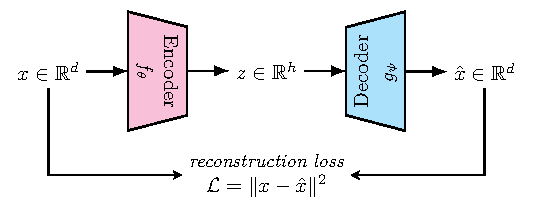
\includegraphics{10/1.pdf}
\end{center}

    The learned representation $z$ can be used for downstream tasks such as
    dimensionality reduction, clustering, or as a feature input to a classifier.  
    \textbf{However, an AE is \emph{not} a generative model}: it provides no principled
    distribution on $z$ to sample from, so generating a new realistic $x$ is not
    guaranteed.

\section{Latent-Variable Generative Modeling}
We now move from representation learning to generative modeling.  
Let $\mathcal D=\{x_i\}_{i=1}^n$ be an unlabeled dataset (e.g.\ images).  
Our goal is to learn a model that can generate \emph{new} data similar to the
training distribution. That is, we want to learn(or equivalently, approximate) a model $p_\theta(x)$ that can generate new data similar to the training distribution.

The key idea is to introduce a latent variable $z$ with a simple prior $p(z)$,
and generate $x$ via a conditional distribution $p_\theta(x\mid z)$ whose
parameters are produced by a neural network.

\begin{definition}[Latent-variable generative model]\label{def:vae-lvm}
    Choose a prior $p(z)$ (easy to sample), and a conditional likelihood
    $p_\theta(x\mid z)$ (expressive).  The marginal model is
    \begin{equation}\label{eq:vae-marginal}
        p_\theta(x)=\int p_\theta(x\mid z)\,p(z)\,\mathrm dz.
    \end{equation}
\end{definition}
\begin{note}
    That is, $p_\theta(x)$ is the integral of $p_\theta(x\mid z)$ with measure $p(z)$.
\end{note}

A canonical choice is the standard Gaussian prior $p(z)=\mathcal N(0,I),$
and an isotropic Gaussian likelihood whose mean is a neural network:
\begin{equation}\label{eq:vae-decoder-gauss}
    p_\theta(x\mid z)=\mathcal N\!\bigl(x\mid f_\theta(z),\,\sigma^2 I\bigr).
\end{equation}
\begin{center}
    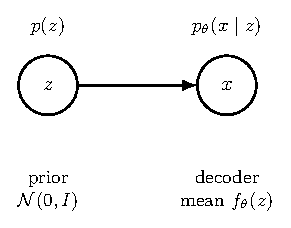
\includegraphics{10/2.pdf}
\end{center}
\begin{note}
    It is absolutely not necessary to use a Gaussian likelihood. Any distribution that is not ill-conditioned is suitable. Here we use a Gaussian likelihood only for simplicity.
\end{note}

\begin{remark}
    If $f_\theta$ were linear, then $x$ would remain Gaussian.  
    A nonlinear and expressive $f_\theta$ enables highly non-Gaussian and complex
    distributions over $x$.
\end{remark}

The maximum-likelihood objective is
\begin{equation}\label{eq:vae-mle}
    \argmax_\theta\;\sum_{i=1}^n \log p_\theta(x_i).
\end{equation}
But expanding \eqref{eq:vae-marginal} gives
\begin{equation}\label{eq:vae-mle-integral}
    \log p_\theta(x)
    =
    \log\int p_\theta(x\mid z)\,p(z)\,\mathrm dz,
\end{equation}
where the integral is typically intractable when $p_\theta(x\mid z)$ is defined
by a deep neural network.
One may try the Monte Carlo approximation
\begin{equation}
    p_\theta(x)
    \approx
    \frac{1}{K}\sum_{k=1}^K p_\theta\bigl(x\mid z^{(k)}\bigr),
    \qquad z^{(k)}\sim p(z),
\end{equation}
i.e., estimate the marginal likelihood by sampling latent codes from the prior and
averaging the corresponding conditional likelihoods. In principle this is valid,
but in high dimensions most prior samples $z^{(k)}$ will fall in regions that are
unlikely to explain a specific datapoint $x$. Consequently, the terms
$p_\theta(x\mid z^{(k)})$ are typically extremely small for most samples, and the
average is dominated by rare lucky valid samples. This leads to very large variance,
so obtaining a reliable estimate would require a large $K$ {for each datapoint}
$x_i$, which quickly becomes computationally prohibitive.

Since this is a latent-variable model, one may also consider the EM algorithm.
Recall that EM alternates between (i) inferring the latent variable distribution
given the current parameters (E-step) and (ii) maximizing the expected complete-data
log-likelihood under that inferred distribution (M-step). Concretely, the E-step
requires the posterior
\begin{equation}
    p_\theta(z\mid x)
    =
    \frac{p_\theta(x\mid z)p(z)}{p_\theta(x)}
    \propto p_\theta(x\mid z)p(z),
\end{equation}
because the M-step depends on expectations taken with respect to $p_\theta(z\mid x)$.
However, the normalization constant is exactly the marginal likelihood
$p_\theta(x)=\int p_\theta(x\mid z)p(z)\,dz$, which is the same intractable integral
as in \eqref{eq:vae-mle-integral}. In classical mixture models (e.g., MoG), the latent
variable is discrete, so the corresponding normalization is a finite sum and the
posterior can be computed exactly; in VAE, $z$ is continuous and high-dimensional,
so the required integrals are generally intractable.

\textbf{The essential bottleneck, therefore, is that we cannot evaluate or sample from the
true posterior $p_\theta(z\mid x)$ efficiently.} Variational inference addresses this
by replacing the intractable posterior with a tractable approximation
\begin{equation}
    q_\phi(z\mid x)\approx p_\theta(z\mid x),
\end{equation}
where $q_\phi$ is chosen from a convenient family (e.g., Gaussians with diagonal
covariance) and its parameters are produced by another neural network, called the
\emph{encoder}. Intuitively, instead of performing an exact E-step, we learn an
inference model that takes a datapoint $x$ as input and outputs a distribution
over plausible latent codes $z$ that could have generated $x$ under the decoder.
\begin{remark}
    Actually, sampling a random number itself is not easy. Even producing a single
    sample that is close to uniform on the interval $[0,1]$ already relies on
    carefully designed pseudo-random number generators and deterministic
    transformations. Sampling from a more complex distribution, especially one
    defined on a high-dimensional space or on a complicated manifold, is therefore
    substantially more challenging.
\end{remark}

\begin{theorem}[ELBO decomposition]\label{thm:vae-elbo-decomp}
For any distribution $q_\phi(z\mid x)$,
\begin{equation}\label{eq:vae-elbo-decomp}
    \log p_\theta(x)
    =
    \underbrace{
    \mathbb E_{z\sim q_\phi(\cdot\mid x)}\!\bigl[\log p_\theta(x\mid z)\bigr]
    -
    \mathrm{KL}\!\left(q_\phi(z\mid x)\,\middle\|\,p(z)\right)
    }_{\mathcal L_{\mathrm{ELBO}}(x;\theta,\phi)}
    +
    \underbrace{
    \mathrm{KL}\!\left(q_\phi(z\mid x)\,\middle\|\,p_\theta(z\mid x)\right)
    }_{\ge 0}.
\end{equation}
Hence $\mathcal L_{\mathrm{ELBO}}(x;\theta,\phi)\le \log p_\theta(x)$.
\end{theorem}
\begin{remark}
    In \eqref{eq:vae-elbo-decomp}, the two KL divergences are different and should
    not be confused. The KL term inside the ELBO compares $q_\phi(z\mid x)$ with
    the prior $p(z)$, while the remaining KL term measures the gap between
    $q_\phi(z\mid x)$ and the true posterior $p_\theta(z\mid x)$.
\end{remark}

\begin{remark}
    The KL term \(\mathrm{KL}(q_\phi(z\mid x)\|p(z))\) \emph{appears inside} ELBO and acts as
    a regularizer toward the prior.  
    The KL term \(\mathrm{KL}(q_\phi(z\mid x)\|p_\theta(z\mid x))\) is the \emph{gap} between
    ELBO and the true log-evidence \(\log p_\theta(x)\).
\end{remark}
    During optimization, we 
    optimize $\log p_\theta(x)$ indirectly by maximizing a tractable lower bound
    (the ELBO). (Because the gap is intractable)

    Although the gap term $\mathrm{KL}\!\left(q_\phi(z\mid x)\,\middle\|\,p_\theta(z\mid x)\right)$
    cannot be optimized explicitly, both $q_\phi$ and $p_\theta$ depend on the
    parameters $(\phi,\theta)$ and are updated jointly when maximizing the ELBO.
    As a result, the gap is implicitly affected during training and does not
    remain fixed or uncontrolled.

The expectation in $\mathbb E_{q_\phi(z\mid x)}[\log p_\theta(x\mid z)]$ still
involves an integral, but the sampling distribution is now data-dependent.
This is a major improvement: the most costly part in practice is drawing
informative samples, and sampling from the prior is inefficient. By replacing
prior sampling with sampling conditioned on the observed data, the computation
is focused on latent regions that actually explain $x$.
Instead of drawing samples from the broad prior $p(z)=\mathcal N(0,I)$, we sample
from the posterior $q_\phi(z\mid x)$, which typically concentrates its mass in a
narrow region relevant to the given data point. As a result, Monte Carlo
estimates of the expectation can have significantly lower variance.
\begin{figure}[h]
    \centering
    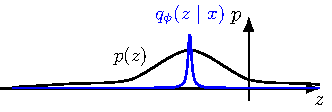
\includegraphics{10/4.pdf}
    \caption{A narrow $q_\phi(z\mid x)$ concentrates its mass in a relatively narrow region, while a broad $p(z)$ has a wide distribution.}
    \label{fig:vae-kl-regularization}
\end{figure}
\begin{note}
    From the perspective of information theory, the condition $x$ brings additional information about $z$, which increase the success probability of sampling a valid, meaningful $z$.
\end{note}
\begin{note}
    The prior $p(z)$ does not participate in training by being sampled in the forward
optimization path. Instead, it enters training through the KL regularization
term, which constrains and aligns the overall shape of $q_\phi(z \mid x)$.
Meanwhile, by sampling $z \sim q_\phi(z \mid x)$ and reconstructing $x$, the model
is forced during self-optimization to maintain stable decoding within a
neighborhood around $\mu_\phi(x)$, thereby endowing the latent representation
with semantic consistency and smoothness.

The weight of the KL term must be balanced. If the KL term is too small,
$q_\phi(z \mid x)$ tends toward deterministic encoding ($\sigma \to 0$), and the
latent space lacks a well-structured global organization, leading to poor
interpolation and unreliable sampling from the prior. If the KL term is too
large, $q_\phi(z \mid x)$ is pushed close to $p(z)$, and the latent variables carry
insufficient information about $x$, making it difficult for the decoder to
recover meaningful samples. These two cases correspond respectively to an
irregular latent space and information collapse.
\begin{center}
    
\includegraphics{10/5.pdf}
\end{center}
\end{note}
Training VAE maximizes the ELBO over the dataset:
\begin{equation}\label{eq:vae-max-elbo}
    \argmax_{\theta,\phi}\;\sum_{i=1}^n \mathcal L_{\mathrm{ELBO}}(x_i;\theta,\phi).
\end{equation}

Assume the decoder likelihood \eqref{eq:vae-decoder-gauss}.  
Then, up to an additive constant independent of $\theta$,
\begin{equation}\label{eq:vae-loglik-mse}
    \log p_\theta(x\mid z)
    =
    -\frac{1}{2\sigma^2}\bigl\|x-f_\theta(z)\bigr\|^2 + C.
\end{equation}
Plugging this into \eqref{eq:vae-elbo-decomp}, maximizing ELBO is equivalent to
minimizing (ignoring constants)
\begin{equation}\label{eq:vae-min-form}
    \argmin_{\theta,\phi}\;
    \sum_{i=1}^n
    \left[
        \mathbb E_{z\sim q_\phi(\cdot\mid x_i)}
        \bigl\|x_i-f_\theta(z)\bigr\|^2
        +
        \beta\,
        \mathrm{KL}\!\left(q_\phi(z\mid x_i)\,\middle\|\,p(z)\right)
    \right],
\end{equation}
where $\beta=2\sigma^2$ (or we may treat $\beta$ as a tunable weight, leading to
\(\beta\)-VAE).

\begin{remark}
    If we remove the KL regularization term, \eqref{eq:vae-min-form} becomes a
    standard autoencoder objective: it reconstructs well but does not enforce a
    tractable sampling distribution in latent space, hence is not a principled
    generative model.
\end{remark}

The KL regularizer encourages $q_\phi(z\mid x)$ to be close to the fixed prior
$p(z)=\mathcal N(0,I)$.  
After training, to \emph{generate} a new sample, we do not need the encoder:
\begin{equation}
    z\sim p(z),\qquad x\sim p_\theta(x\mid z).
\end{equation}
Because $p(z)$ is simple to sample and the decoder is learned, we can generate
new $x$.

\begin{note}
    In modern diffusion systems, VAE is often used as a \emph{latent
    autoencoder}, diffusion operates in the latent space, then the VAE decoder
    maps latent variables back to pixel space.
\end{note}

\section{Reparameterization Trick}
To optimize \eqref{eq:vae-min-form} with backpropagation, we must be able to
compute gradients with respect to the encoder parameters $\phi$. However, if we
sample directly by $z\sim q_\phi(z\mid x),$
then $z$ is produced by a stochastic sampling operation rather than an explicit
differentiable function of $\phi$. In other words, small changes in $\phi$ change
the distribution $q_\phi(z\mid x)$, but the random draw $z$ itself does not provide
a differentiable path for gradients to flow back to $\phi$, which breaks
end-to-end training.

A standard choice is to let the encoder output a Gaussian distribution
\begin{equation}\label{eq:vae-encoder-gauss}
    q_\phi(z\mid x)=\mathcal N\!\bigl(z\mid \mu_\phi(x),\,\Sigma_\phi(x)\bigr),
\end{equation}
often with diagonal covariance
\begin{equation}
    \Sigma_\phi(x)=\mathrm{diag}\bigl(\sigma_\phi^2(x)\bigr).
\end{equation}

Sample instead from a parameter-free noise distribution:
\begin{equation}
    \varepsilon\sim \mathcal N(0,I),
    \qquad
    z=\mu_\phi(x) + L_\phi(x)\,\varepsilon,
\end{equation}
where $L_\phi(x)L_\phi(x)^\top=\Sigma_\phi(x)$ (for diagonal covariance,
$L_\phi(x)=\mathrm{diag}(\sigma_\phi(x))$).

\begin{proposition}[Correctness of reparameterization]\label{prop:vae-reparam}
If $\varepsilon\sim\mathcal N(0,I)$ and $z=\mu + L\varepsilon$, then
$z\sim\mathcal N(\mu,LL^\top)$.
\end{proposition}
\begin{proof}
The affine transformation of a Gaussian remains Gaussian.  
Moreover,
\begin{equation}
    \mathbb E[z]=\mu + L\,\mathbb E[\varepsilon]=\mu,
\end{equation}
and
\begin{equation}
    \mathrm{Cov}(z)
    =
    L\,\mathrm{Cov}(\varepsilon)\,L^\top
    =
    LIL^\top
    =
    LL^\top.
\end{equation}
\end{proof}

    The sampling step now occurs in $\varepsilon$, which has no learnable
    parameters; gradients only need to flow through differentiable operations
    producing $\mu_\phi(x)$ and $L_\phi(x)$.
\begin{note}
    In a deterministic autoencoder, each data point $x$ is mapped to a single latent
code $z$, and the reconstruction loss only enforces correctness at that
particular point. The decoder is therefore unconstrained in the neighborhood
around $z$.

In contrast, a VAE represents each data point by a Gaussian
distribution $q_\phi(z\mid x)=\mathcal N(\mu(x),\sigma^2(x))$. During training,
latent variables are sampled from this distribution. As a result, the decoder is
required to reconstruct x not just at a single latent code, but throughout a
neighborhood around $\mu(x)$. This stochasticity induces a smooth latent space.
\end{note}
\begin{figure}[h]
    \centering
    
\includegraphics{10/3.pdf}
    \caption{The structure of a VAE, in which orange KL loss is regularized towards the prior $p(z)$ which is trained for sampling during generation, and the cyan ELBO loss is regularized towards the decoder $p_\theta(x\mid z)$. The source of randomness is shifted from sampling $z$ itself to sampling an
    auxiliary variable $\varepsilon$, so that $z$ becomes a deterministic function
    of $\varepsilon$ and the parameters. As a result, the gradient paths through the
    functions of $z$ in both $p_\theta$ and $q_\phi$ are preserved.}
    \label{fig:vae-structure}
\end{figure}
The KL term in \eqref{eq:vae-min-form} is tractable when both distributions are
Gaussian.
\begin{theorem}[Gaussian--Gaussian KL]\label{thm:vae-kl-gauss}
Let \(q=\mathcal N(\mu,\Sigma)\) and \(p=\mathcal N(0,I)\). Then
\begin{equation}\label{eq:vae-kl-gauss}
    \mathrm{KL}(q\|p)
    =
    \frac{1}{2}\Bigl(
        \mathrm{tr}(\Sigma) + \mu^\top \mu - d - \log\det(\Sigma)
    \Bigr).
\end{equation}
In the diagonal case $\Sigma=\mathrm{diag}(\sigma_1^2,\dots,\sigma_d^2)$, this becomes
\begin{equation}\label{eq:vae-kl-diag}
    \mathrm{KL}(q\|p)
    =
    \frac{1}{2}\sum_{j=1}^d
    \left(
        \mu_j^2 + \sigma_j^2 - 1 - \log \sigma_j^2
    \right).
\end{equation}
\end{theorem}

\begin{remark}
    Therefore, VAE training typically uses:
    \begin{itemize}
        \item a decoder network $f_\theta$ for $p_\theta(x\mid z)$;
        \item an encoder network producing two ``heads'': $\mu_\phi(x)$ and
        $\log \sigma_\phi^2(x)$;
        \item one (or a few) Monte Carlo samples per datapoint for the
        reconstruction expectation.
    \end{itemize}
\end{remark}

\end{document}